% ================================================================ 13
\section{Proceso de compilación}

El proceso de compilación de \ggez\ consiste en cuatro fases que analizan el código fuente, a partir del archivo principal, para detectar cualquier error antes de permitir su ejecución. Esta sección describe las fases del compilador y las herramientas que lo implementan.

\subsection{Fases del compilador}

\textbf{1. Análisis léxico} (\kw{lexer.py}). El código fuente se convierte en una secuencia de tokens: palabras reservadas, identificadores, literales y símbolos. Se descartan los comentarios y se emite un fin de línea por cada salto, excepto dentro de un \kw{\{} o un \kw{<} sin cerrar. Se detectan errores léxicos como caracteres no reconocidos, cadenas sin cerrar o nombres con tilde.

\textbf{2. Análisis sintáctico} (\kw{sintactico.py}). Un analizador descendente recursivo, con una función por cada regla de la gramática, organiza los tokens en un árbol sintáctico (\kw{arbol.py}). Se detectan errores sintácticos como bloques sin \kw{gg}, palabras fuera de orden, un \kw{combo} sin \kw{drops} o expresiones incompletas.

\textbf{3. Resolución de importaciones} (\kw{cargador.py}). A partir del archivo principal se sigue cada \kw{travel} en profundidad: cada archivo importado se analiza léxica y sintácticamente, se verifica que no tenga \kw{lobby.launch} y que no se repita un módulo, y se detectan las importaciones circulares llevando el camino de archivos que se están cargando. Cada archivo se carga una sola vez.

\textbf{4. Análisis semántico} (\kw{semantico.py}). Sobre los árboles de todos los archivos, con una tabla de símbolos por alcance, se verifican: el punto de entrada único, las declaraciones y redeclaraciones, el sombreado, los tipos de cada expresión, asignación y retorno, la cantidad y el tipo de los argumentos (también de los \kw{combo} importados), la visibilidad y la herencia de las clases, las constantes, que todo camino de un \kw{combo} con retorno termine en \kw{reward} y que \kw{ragequit} y \kw{respawn} estén dentro de un ciclo. En esta fase también se calculan las advertencias.

\subsection{Herramientas técnicas}

El compilador está escrito en Python 3, sin bibliotecas externas: el analizador léxico, el sintáctico, el cargador de importaciones y el analizador semántico se implementaron a mano. Se eligió escribir el analizador sintáctico como descendente recursivo porque cada función corresponde a una regla de la gramática de \kw{GRAMATICA.md}, lo que facilita leerlo, mantenerlo y producir mensajes de error propios en español. Las palabras reservadas están definidas en un único archivo (\kw{tokens.py}), de modo que cambiar una palabra del lenguaje se hace en un solo lugar.

El compilador se usa desde el IDE o desde la línea de comandos:

\begin{longtable}{|p{4.6cm}|p{9.8cm}|}\hline
\cab\textbf{Comando} & \textbf{Uso} \\\hline\endhead
\kw{ggezc compile <archivo>} & Valida el proyecto completo (fases 1 a 4) sin ejecutar. \\\hline
\kw{ggezc run <archivo>} & Valida y, si no hay errores, ejecuta. \\\hline
\kw{ggezc check <archivo>} & Corre las pruebas del \kw{nivel.json} de la carpeta (modo de juego). \\\hline
\kw{ggezc tokens <archivo>} & Muestra los tokens del análisis léxico. \\\hline
\kw{--pasos N} & Cambia la cantidad de maná (por defecto 5\,000\,000). \\\hline
\kw{--eventos} & Emite las líneas \kw{@ggez} que el IDE usa para el modo de juego. \\\hline
\end{longtable}

\begin{lstlisting}[language={}]
$ python ggezc.py compile principal.ggez
Compilacion exitosa: principal.ggez y 2 archivo(s) importado(s)
\end{lstlisting}

\subsection{Reporte de errores}

Cuando el compilador detecta un error en cualquiera de las fases, la compilación se detiene y se reporta ese único error. Al corregirlo y volver a compilar aparece el siguiente, si lo hay. Así el estudiante se concentra en un problema a la vez, en lugar de una lista larga de errores que muchas veces son consecuencia del primero. El error se escribe en la salida de errores con el formato estándar (sección~\ref{sec:errores}) y el IDE lo muestra en la pestaña Problemas. Si el proyecto compila, se reportan además sus advertencias, que no impiden ejecutar.

\newpage
% ================================================================ 14
\section{Proceso de ejecución}

Una vez que la compilación termina sin errores, el intérprete ejecuta el programa. Esta sección describe la estrategia del intérprete y cómo gestiona el estado del programa.

\subsection{Estrategia general}

El intérprete de \ggez\ (\kw{evaluador.py}) recorre directamente el árbol sintáctico y ejecuta cada nodo según su tipo (\emph{tree-walking interpreter}). No genera código intermedio ni usa \kw{eval} o \kw{exec} de Python. Este enfoque es sencillo de implementar y adecuado para el propósito educativo del lenguaje.

\subsection{Flujo de ejecución}

\begin{itemize}
  \item Al presionar Ejecutar (\kw{F5}), el IDE guarda todos los archivos y ejecuta el archivo \kw{.ggez} de la pestaña enfocada; si la pestaña enfocada no es un \kw{.ggez}, usa el archivo principal del proyecto. Si el archivo está en una carpeta de nivel, corre las pruebas del nivel en vez de ejecutarlo.
  \item El IDE lanza \kw{ggezc run} en una terminal integrada libre, con la carpeta del proyecto como directorio de trabajo.
  \item El traductor realiza las cuatro fases de compilación. Si hay un error, lo reporta y termina con código 1 sin ejecutar nada.
  \item El intérprete registra los \kw{combo}, \kw{guild} e \kw{inventory} de todos los archivos y ejecuta el bloque de \kw{lobby.launch} instrucción por instrucción.
  \item Las declaraciones y asignaciones actualizan el entorno; las estructuras de control deciden la siguiente instrucción; las llamadas crean un entorno nuevo y transfieren el control al cuerpo de la función. \kw{reward}, \kw{ragequit}, \kw{respawn} y \kw{wipe} se implementan como señales internas que suben hasta la construcción que las maneja.
  \item \kw{chat.send} escribe en la salida estándar, \kw{chat.rage} en la de errores y \kw{chat.load} lee de la entrada estándar. La terminal del IDE está conectada a los tres, por lo que el estudiante escribe sus respuestas directamente en ella.
  \item La ejecución termina al completar el bloque de \kw{lobby.launch}, con un error no atrapado, al agotarse el maná o cuando el usuario la interrumpe con \kw{Ctrl+C} en la terminal. Al terminar, el IDE actualiza el maná, las misiones y los logros.
\end{itemize}

\begin{figure}[H]
\centering
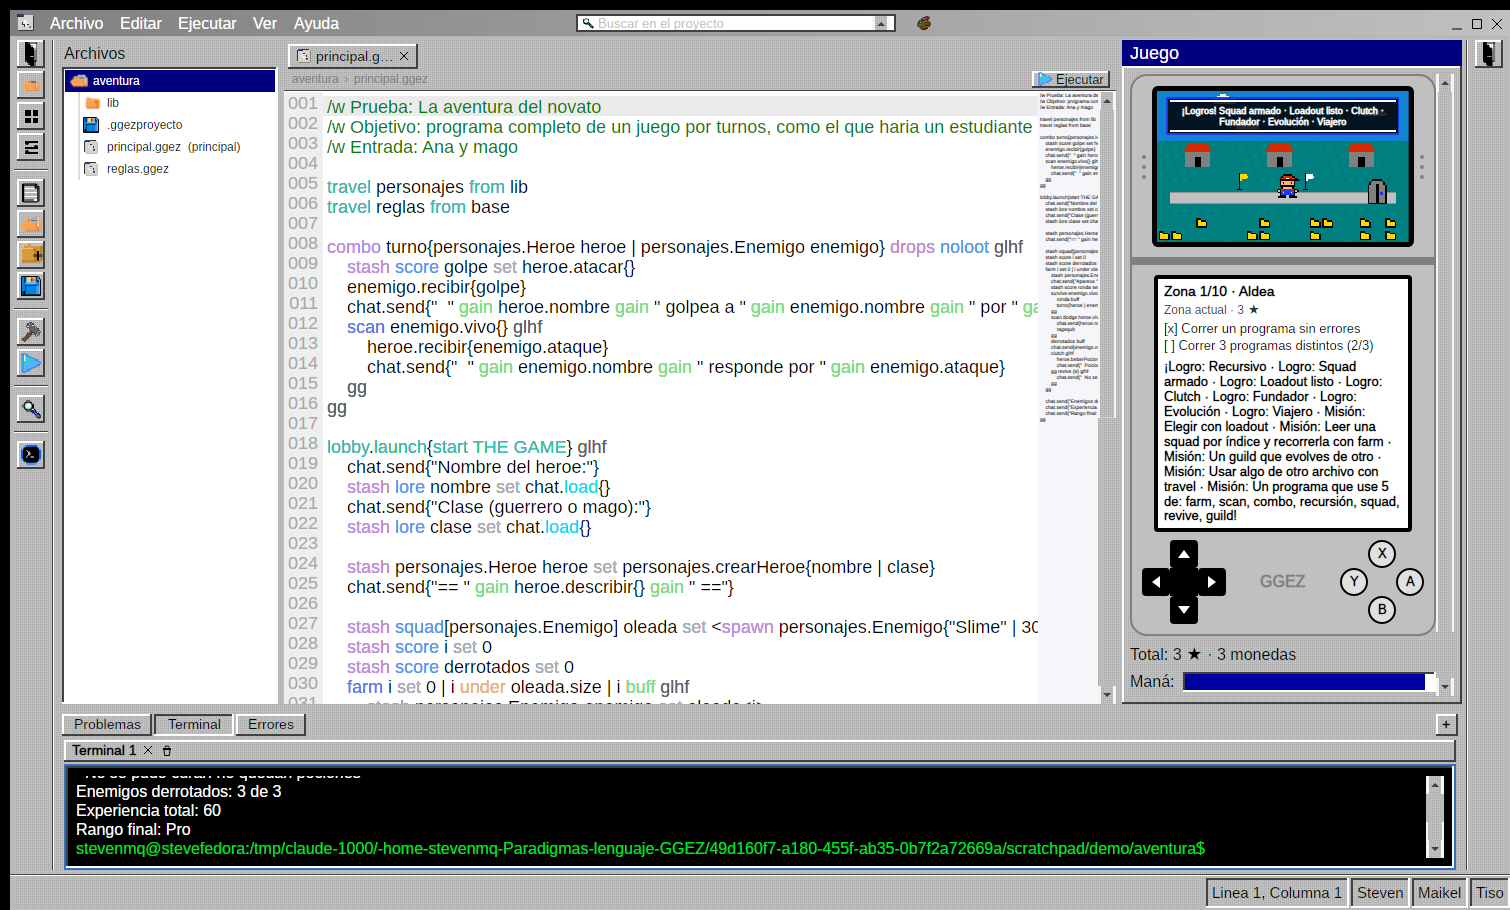
\includegraphics[width=0.92\textwidth]{img/ide_ejecucion.png}
\caption{Ejecución de un programa con entrada interactiva en la terminal integrada.}
\end{figure}

\subsection{Gestión de alcances}

Existe un entorno global con las funciones y tipos de cada archivo. Cada bloque (rama de un \kw{scan}, cuerpo de un ciclo, bloque de \kw{clutch}) crea un entorno hijo que se descarta al llegar a su \kw{gg}. Cada llamada a un \kw{combo} crea un entorno nuevo con sus parámetros, que no ve las variables de quien hizo la llamada. Dentro de un método, los nombres se buscan primero en las variables locales, después en los campos y métodos del objeto y por último en los \kw{combo} globales.

\subsection{Ejecución de importaciones}

Cuando el intérprete encuentra una llamada a un \kw{combo} importado (\kw{modulo.combo\{\}}), ejecuta el cuerpo de esa función con su propio entorno, aislado del archivo que la llamó, y devuelve el valor al punto de la llamada. Lo mismo ocurre con \kw{spawn modulo.Tipo\{\}}. Los archivos importados no ejecutan código propio: solo aportan declaraciones.

\subsection{Limitaciones de la ejecución}

\begin{itemize}
  \item \textbf{Maná.} Cada instrucción y cada vuelta de un ciclo gasta un punto. El programa empieza con 5\,000\,000; si se agota, termina con el error «sin mana». Así un ciclo infinito no congela el IDE. Este error no se puede atrapar con \kw{revive}.
  \item \textbf{Recursión.} La profundidad máxima es de 5000 llamadas anidadas; al superarla se produce un error que indica revisar el caso base.
  \item \textbf{Velocidad.} Un intérprete que recorre el árbol es más lento que un lenguaje compilado a código nativo, lo cual es aceptable para el propósito educativo del lenguaje.
\end{itemize}

\newpage
% ================================================================ 15
\section{Manejo de errores}
\label{sec:errores}

El sistema de manejo de errores es uno de los componentes centrales de \ggez, porque es lo primero que encuentra un principiante cuando algo sale mal. Esta sección documenta las categorías de errores, el formato de los mensajes y el comportamiento del aplicativo.

\subsection{Categorías de errores}

\begin{longtable}{|p{3cm}|p{4.4cm}|p{7cm}|}\hline
\cab\textbf{Categoría} & \textbf{Momento de detección} & \textbf{Ejemplos típicos} \\\hline\endhead
Léxicos & Análisis léxico (fase 1) & Caracteres no reconocidos, cadenas sin cerrar, nombres con tilde \\\hline
Sintácticos & Análisis sintáctico (fase 2) & Bloques sin \kw{gg}, \kw{combo} sin \kw{drops}, punto de entrada mal escrito, falta un valor \\\hline
De importación & Resolución de importaciones (fase 3) y llamadas a lo importado (fase 4) & Archivo o función inexistente, módulo duplicado, importación circular, argumentos incorrectos en una llamada importada \\\hline
Semánticos & Análisis semántico (fase 4) & Variable no declarada, tipos incompatibles, cantidad de argumentos, redeclaración, sin punto de entrada \\\hline
En ejecución & Interpretación del programa & División entre cero, índice fuera de rango, objeto \kw{afk}, \kw{wipe} no atrapado, sin maná, recursión excesiva \\\hline
De proyecto & En el IDE, antes de compilar & La pestaña enfocada no es un \kw{.ggez} y no hay archivo principal, o este fue borrado \\\hline
\end{longtable}

\subsection{Formato estándar de los mensajes}

Cada mensaje de error incluye: (1) el archivo, (2) la línea, (3) la columna, (4) el tipo de error, (5) una descripción del problema y (6) una posible causa. Se escribe en dos líneas:

\begin{lstlisting}[language={}]
principal.ggez:7:25: error semantico: 'escudo' no esta declarada
    posible causa: Declarela con stash antes de usarla, o revise si
    escribio mal el nombre o si quedo en otro bloque.
\end{lstlisting}

Para encontrar la posible causa, el traductor busca en el mensaje fragmentos conocidos (por ejemplo «no esta declarada» o «se obtuvo») y, si ninguno coincide, usa una sugerencia general según el tipo de error. Los mensajes evitan tildes para que se vean bien en cualquier consola.

En el IDE, la pestaña Problemas presenta cada error con su ícono, el archivo y la línea, la descripción y, debajo, la posible causa en gris.

\begin{figure}[H]
\centering
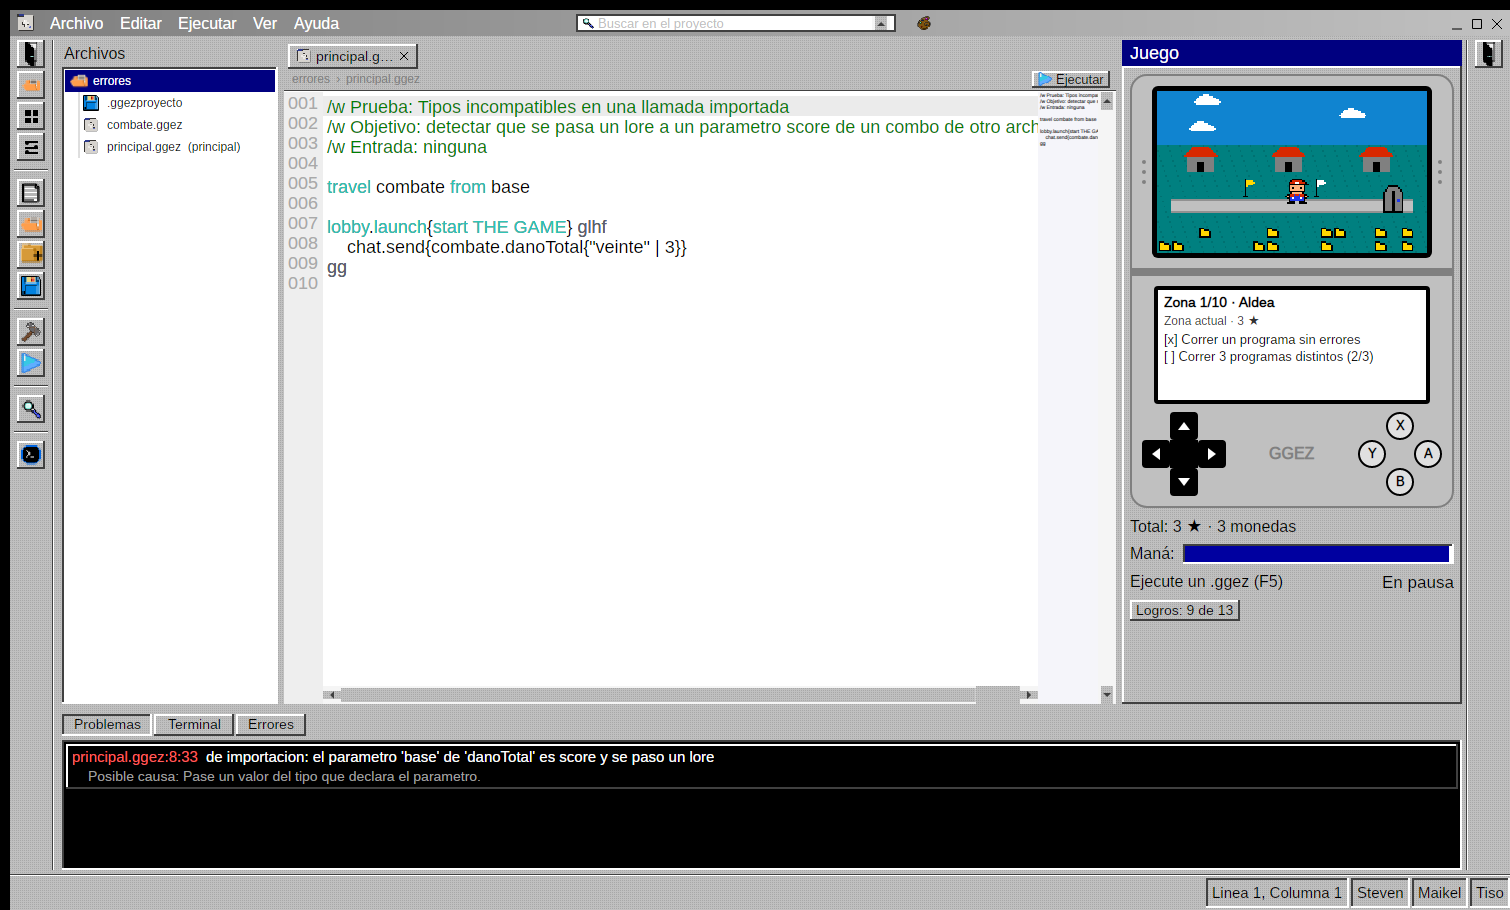
\includegraphics[width=0.92\textwidth]{img/problemas_error.png}
\caption{Pestaña Problemas con un error y su posible causa.}
\end{figure}

\subsection{Filosofía de retroalimentación}

Los mensajes de \ggez\ siguen cuatro principios: (1) \textbf{lenguaje claro}, en español y sin jerga innecesaria; (2) \textbf{ubicación precisa}, con archivo, línea y columna; (3) \textbf{orientación a la solución}, diciendo qué revisar y no solo qué falló; y (4) \textbf{un error a la vez}, para no abrumar.

\subsection{Comportamiento del aplicativo}

Un programa con errores de compilación no se ejecuta. Los errores en ejecución detienen el programa en el punto donde ocurren, salvo que se atrapen con \kw{clutch}/\kw{revive}. En ambos casos la terminal muestra el error en rojo y la pestaña Problemas lo lista; un clic sobre el problema abre el archivo y lleva el cursor a la línea. La pestaña Errores (menú Ejecutar, «Ver errores») conserva los mensajes del IDE. Cada vez que se compila o ejecuta, la pestaña Problemas se limpia y muestra solo el estado actual.

\subsection{Advertencias}

Cuando el programa compila sin errores, el compilador revisa además tres situaciones que no impiden ejecutar pero suelen indicar un descuido:

\begin{longtable}{|p{4cm}|p{10.4cm}|}\hline
\cab\textbf{Advertencia} & \textbf{Cuándo se reporta} \\\hline\endhead
Variable sin usar & Una variable declarada cuyo valor nunca se lee. Asignarle un valor no cuenta como leerla. \\\hline
\kw{combo} sin usar & Un \kw{combo} del archivo principal que nunca se llama; las llamadas a sí mismo no cuentan. Los archivos importados no se revisan, porque pueden tener funciones que el programa no necesita. \\\hline
Código que nunca se ejecuta & Instrucciones escritas después de un \kw{reward}, \kw{ragequit}, \kw{respawn} o \kw{wipe} en el mismo bloque. \\\hline
\end{longtable}

Las advertencias usan el mismo formato que los errores, con el tipo \kw{advertencia}, y el IDE las muestra en amarillo.

\begin{lstlisting}[language={}]
principal.ggez:6:5: advertencia: la variable 'oro' se declaro pero su valor nunca se usa
\end{lstlisting}

\begin{figure}[H]
\centering
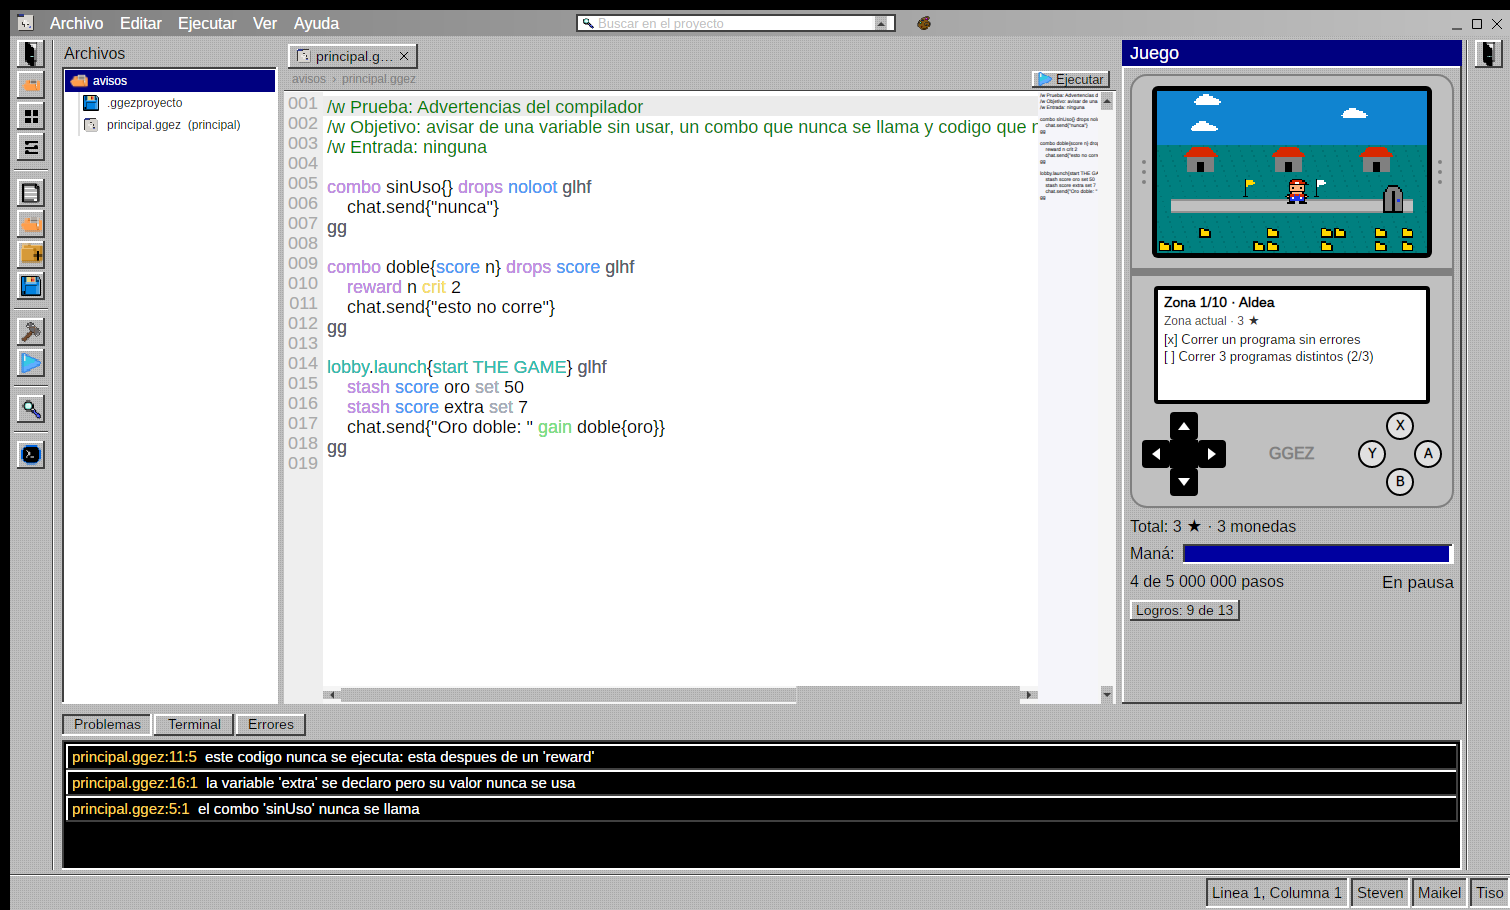
\includegraphics[width=0.92\textwidth]{img/advertencias.png}
\caption{Advertencias en amarillo en la terminal y en la pestaña Problemas.}
\end{figure}

\newpage
% ================================================================ 16
\section{Innovación}
\label{sec:innovacion}

La característica de innovación de \ggez\ es que \textbf{el entorno de desarrollo es en sí mismo un juego}, cuyo progreso depende de que el código del estudiante funcione de verdad. Se complementa con una terminal real con asistente de inteligencia artificial y un sistema de extensiones. Esta sección describe su funcionamiento, cómo se integra con el traductor y por qué se eligió.

\subsection{Descripción funcional}

El IDE tiene un panel de juego, a la derecha del editor, que muestra el maná, el mapa del mundo, el nivel actual, las monedas, las pistas y los logros. Cada vez que el estudiante ejecuta un programa, el traductor informa al IDE cuánto maná gastó, qué construcciones del lenguaje se ejecutaron y si obtuvo algún logro; el IDE actualiza el panel con esa información. Nada se gana con solo escribir código: solo cuenta lo que se ejecutó sin errores.

\subsection{Componentes}

\textbf{Maná.} Cada instrucción y cada vuelta de ciclo gasta un punto de maná, y la barra muestra cuánto gastó el programa. Además de impedir que un ciclo infinito congele el IDE, hace visible el costo de un algoritmo: un programa más eficiente gasta menos.

\textbf{Mundo y misiones.} Un mapa con diez zonas en orden: Aldea, Pradera, Bosque de los ciclos, Río, Cueva, Torre, Mercado, Castillo, Gremio y Guarida del jefe. Cada zona tiene misiones que se cumplen ejecutando programas que usen ciertas construcciones (por ejemplo, un programa con \kw{farm}, \kw{survive} y \kw{grind}, o uno con un \kw{guild} que \kw{evolves} de otro). Al completar las misiones de una zona se abre la siguiente.

\begin{figure}[H]
\centering
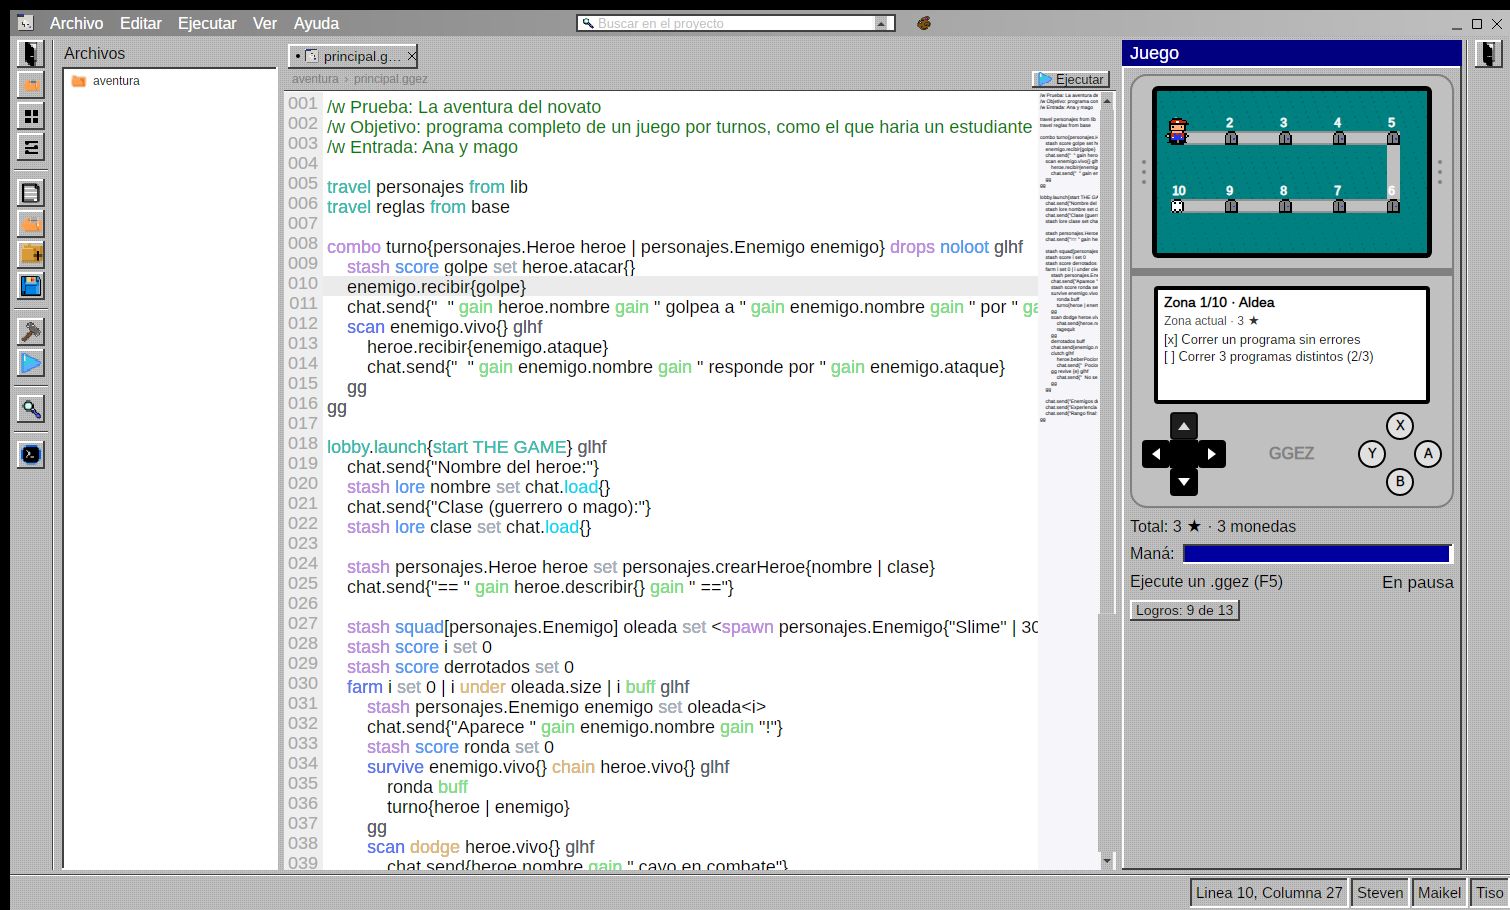
\includegraphics[width=0.8\textwidth]{img/mapa.png}
\caption{Mapa del mundo con la zona actual y sus misiones.}
\end{figure}

\textbf{Niveles y estrellas.} Una carpeta con un archivo \kw{nivel.json} define un reto: título, pruebas (una llamada o una entrada, con su salida esperada), pistas y una meta de pasos. Al ejecutar, el traductor corre las pruebas y el IDE otorga hasta tres estrellas: una por pasar todas las pruebas, otra por lograrlo al primer intento y otra por no superar la meta de pasos. Cualquier docente puede crear niveles nuevos con un archivo de texto, sin tocar el código del IDE.

\begin{lstlisting}[language={}]
{
  "titulo": "Suma de Gauss",
  "meta_pasos": 5,
  "pistas": ["Con un farm de 1 a n y boost se pasan las pruebas", "..."],
  "pruebas": [
    { "llamada": "sumarHasta{10}", "salida": "55" },
    { "llamada": "sumarHasta{0}",  "salida": "0" }
  ]
}
\end{lstlisting}

\textbf{Monedas y pistas.} Cada estrella ganada da una moneda, y cada pista de un nivel cuesta una. El estudiante decide si pide ayuda o lo intenta solo.

\textbf{Logros.} Trece logros reconocen hitos de aprendizaje: correr el primer programa sin errores, declarar un \kw{combo}, escribir una recursión, usar \kw{squad}, usar \kw{loadout}, usar los tres ciclos en un programa, atrapar un error, declarar un \kw{guild}, usar herencia, importar un archivo, quedarse sin maná, ganar tres estrellas en un nivel y comprar una pista. Al obtener uno, el IDE muestra una notificación.

\textbf{Temas desbloqueables.} Las estrellas desbloquean temas visuales para el editor (con 6, 15 y 25 estrellas), además de un modo oscuro disponible desde el inicio.

\textbf{Terminal real con asistente de inteligencia artificial.} El segmento de salida admite hasta cuatro terminales en columnas, con comandos propios (\kw{cd}, \kw{clear}, \kw{exit}, \kw{help}). Al instalar la extensión de Claude, las terminales pasan a ser terminales reales del sistema operativo, capaces de correr cualquier programa interactivo, entre ellos el asistente \kw{claude}. Así el estudiante puede pedir, dentro del mismo IDE, que le expliquen un error o un concepto.

\textbf{Sistema de extensiones.} Desde la vista de extensiones se instalan y desinstalan complementos: sangría de colores, resaltado de espacios al final de la línea, resaltado de \kw{TODO}, colores por nivel de bloques, modo oscuro, bloques al estilo Pac-Man, la terminal de Claude y los temas desbloqueables.

\begin{figure}[H]
\centering
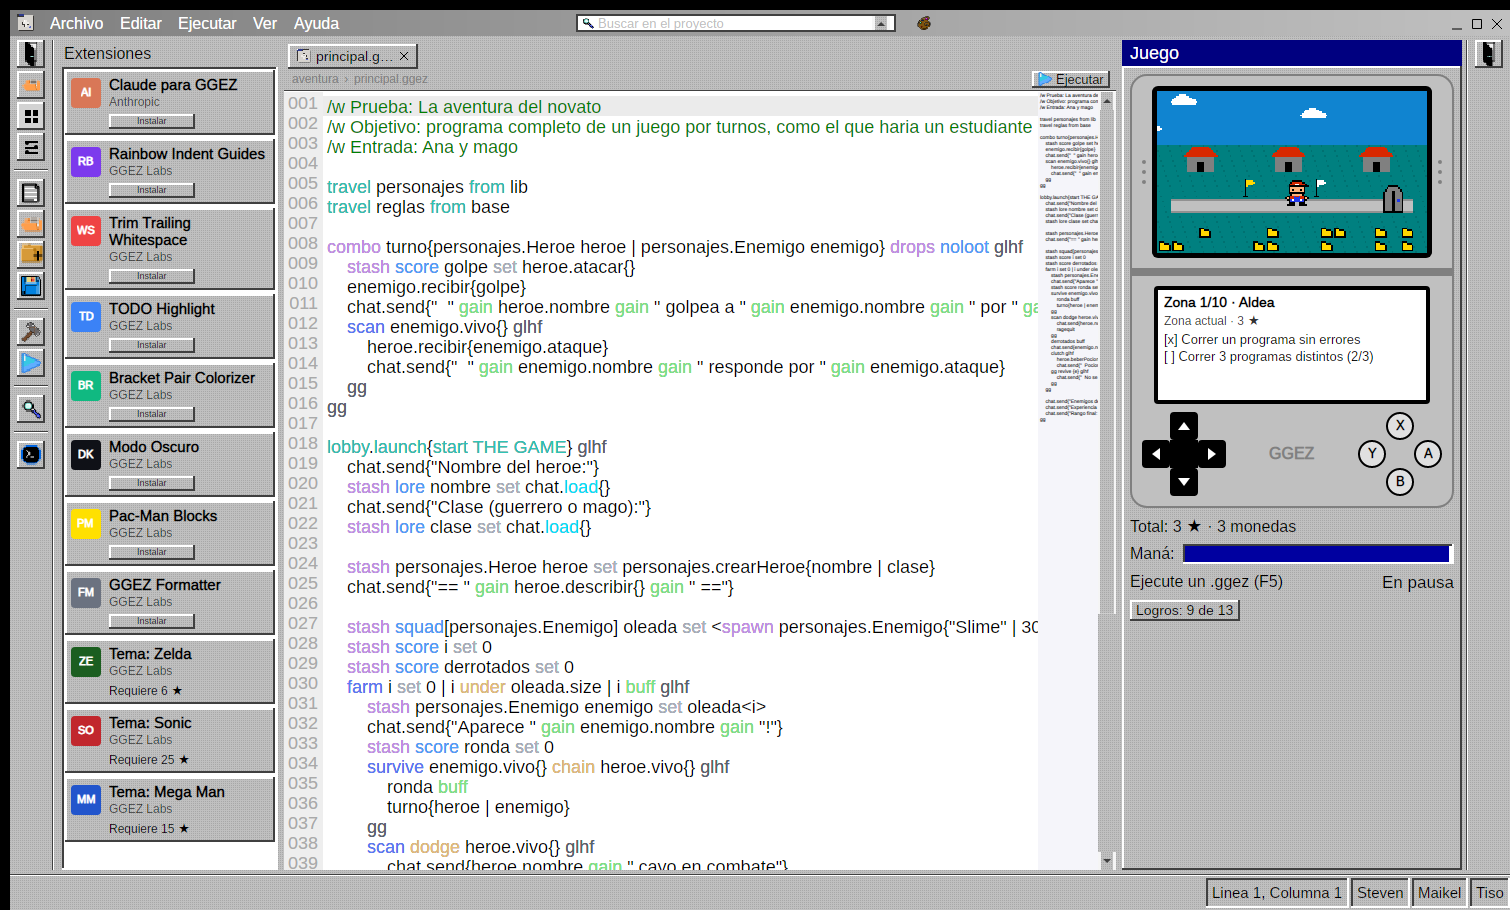
\includegraphics[width=0.92\textwidth]{img/extensiones.png}
\caption{Vista de extensiones.}
\end{figure}

\subsection{Funcionamiento técnico}

El IDE ejecuta el traductor con la opción \kw{--eventos}. Al terminar el programa, el traductor escribe en la salida líneas que empiezan con \kw{@ggez}, que el IDE no muestra en la terminal sino que envía al panel de juego:

\begin{longtable}{|p{5.4cm}|p{9cm}|}\hline
\cab\textbf{Evento} & \textbf{Significado} \\\hline\endhead
\kw{@ggez pasos <usados> <limite>} & Maná gastado y maná disponible. \\\hline
\kw{@ggez logro <id>} & El programa cumplió las condiciones de un logro. \\\hline
\kw{@ggez programa <huella> <usos>} & Huella del programa y construcciones que se ejecutaron (ciclos, recursión, clases, importaciones...), para avanzar las misiones. \\\hline
\kw{@ggez nivel <pasadas> <total> <pasos> <meta> <titulo>} & Resultado de las pruebas de un nivel, para calcular las estrellas. \\\hline
\end{longtable}

Las construcciones usadas se registran durante la ejecución, no al leer el código: un \kw{farm} que nunca dio una vuelta no cuenta. La huella identifica el programa, de modo que una misión que pide varios programas distintos no se cumple ejecutando el mismo dos veces. El progreso (estrellas, monedas, logros, misiones y récords de cada nivel) se guarda en el archivo \kw{progreso.json} de la carpeta de configuración del usuario.

\subsection{Validaciones e integración}

\begin{itemize}
  \item El archivo \kw{nivel.json} puede venir de otra persona, por lo que el traductor revisa su forma antes de usarlo (título de texto, meta de pasos entera y positiva, al menos una prueba con su salida, llamadas de una sola línea) y reporta un error claro si algo está mal.
  \item Un evento con un identificador que el IDE no conoce se ignora.
  \item Solo se puede comprar una pista si hay monedas suficientes y quedan pistas en el nivel.
  \item La gamificación no requiere configuración: funciona desde la primera ejecución y no interfiere con el programa, cuya salida se ve completa en la terminal.
\end{itemize}

\subsection{Justificación}

La elección de esta característica responde a tres consideraciones. Primero, atiende directamente el problema planteado: el estudiante de primer ingreso conoce los videojuegos y su sistema de progreso, y el IDE usa ese mismo lenguaje para mostrarle que está avanzando. Segundo, está ligada al aprendizaje real, porque solo avanza con código que se ejecuta y premia construcciones concretas del lenguaje, por lo que no es un adorno separado de la programación. Tercero, es demostrable durante la presentación: basta ejecutar un programa para ver cómo cambia el maná, se cumple una misión o aparece un logro.

\newpage
% ================================================================ 17
\section{Arquitectura del aplicativo}

El aplicativo tiene dos componentes que se comunican mediante procesos: el \textbf{IDE}, escrito en C\# con Avalonia, y el \textbf{traductor}, escrito en Python. Esta sección describe las tecnologías utilizadas, la organización en capas y los módulos del código fuente.

\subsection{Tecnologías utilizadas}

\begin{itemize}
  \item \textbf{C\# y .NET.} Lenguaje y plataforma del IDE.
  \item \textbf{Avalonia.} Biblioteca de interfaz gráfica multiplataforma que permite que el mismo IDE funcione en Linux y Windows.
  \item \textbf{CommunityToolkit.Mvvm.} Implementa el patrón Modelo-Vista-VistaModelo con propiedades observables y comandos.
  \item \textbf{RoyalTerminal.} Control de terminal que usa la extensión de Claude para ofrecer terminales reales.
  \item \textbf{Python 3.} Lenguaje del traductor, sin bibliotecas externas.
  \item \textbf{Python portátil (python-build-standalone).} Intérprete de Python que se incrusta en el ejecutable para que el usuario no tenga que instalarlo.
  \item \textbf{Nix.} El repositorio incluye un \kw{flake.nix} para preparar el entorno de desarrollo.
  \item \textbf{Git y GitHub.} Control de versiones y trabajo en equipo.
\end{itemize}

\subsection{Organización en capas}

\textbf{Capa de presentación (IDE).} Contiene todo lo visual: ventana principal, menús, árbol de archivos, editor, terminales, pestañas de errores y problemas, panel de juego, ayuda, extensiones y ajustes. Sigue el patrón MVVM: las vistas (\kw{.axaml}) solo muestran datos y los modelos de vista (\kw{ViewModels}) contienen la lógica de la interfaz.

\textbf{Frontera de integración.} El IDE y el traductor solo se comunican por texto: el IDE lanza \kw{ggezc} como un proceso, le pasa la entrada del usuario y lee su salida. Los errores tienen un formato fijo (\kw{archivo:linea:columna: tipo: mensaje}) que el IDE interpreta con una expresión regular, y los eventos del juego empiezan con \kw{@ggez}. Gracias a esto, el traductor puede usarse y probarse sin el IDE.

\textbf{Capa de lógica del lenguaje (traductor).} Contiene el compilador, el intérprete, las pruebas de niveles y los eventos del juego. No depende de la interfaz gráfica.

\textbf{Capa de servicios.} En el IDE, componentes de apoyo: diálogos, configuración, persistencia de la sesión y de las extensiones, temas, progreso del juego, procesos de las terminales e instalación del traductor incrustado.

\subsection{Estructura de módulos}

\begin{lstlisting}[language={}]
ParadigmasLenguajePropio/src/ParadigmasLenguajePropio/   (IDE)
    Views/          ventana, menu, barra de estado, explorador, extensiones,
                    ajustes, editor, terminal, panel de juego
    ViewModels/     logica de cada vista (abrir, guardar, ejecutar, errores)
    Models/         archivos del arbol, problemas, logros, mundo, ayuda
    Services/       dialogos, sesion, temas, progreso, terminales, instalacion
    Controls/       editor (coloreado, autocompletado, minimapa), arbol
    Themes/, Assets/   estilos, fuentes e iconos
Traductor/                                                 (traductor)
    ggezc.py        punto de entrada de la linea de comandos
    GRAMATICA.md    gramatica formal
    src/ggez/
        cli.py          comandos run, compile, check, tokens
        tokens.py       palabras reservadas
        lexer.py        analisis lexico
        sintactico.py   analisis sintactico
        arbol.py        nodos del arbol sintactico
        cargador.py     importaciones con travel
        semantico.py    analisis semantico y advertencias
        evaluador.py    interprete
        errores.py      formato de errores y posible causa
        nivel.py        pruebas de nivel.json
        logros.py       eventos del modo de juego
    pruebas/        casos de la seccion 18 y correr.py
    ejemplos/       programas de ejemplo
publicar.sh         genera el ejecutable unico
\end{lstlisting}

\subsection{Flujo de una operación típica}

Al presionar Compilar (\kw{F6}), el IDE guarda todos los archivos, limpia la pestaña Problemas, toma el archivo \kw{.ggez} enfocado (o el principal, si no hay uno) y lanza \kw{ggezc compile} en una terminal integrada. El traductor ejecuta las cuatro fases de la sección 13 y escribe «Compilacion exitosa» con sus advertencias, o un único error. El IDE lee la salida de errores línea por línea, colorea cada línea según su tipo y llena la pestaña Problemas. Al ejecutar (\kw{F5}) el flujo es el mismo con \kw{ggezc run --eventos}: la salida del programa aparece en la terminal, la entrada del usuario se envía al proceso y, al terminar, los eventos \kw{@ggez} actualizan el panel de juego.

\subsection{Distribución}

El entregable es un ejecutable único por sistema operativo, generado con el script \kw{publicar.sh} de la raíz del repositorio (\kw{./publicar.sh linux}, \kw{windows} o \kw{todo}). El script publica el IDE como un solo archivo y le incrusta un Python portátil y el traductor; la primera vez que se abre, el IDE los despliega en la carpeta de datos del usuario. Así el estudiante no necesita instalar .NET ni Python.

\subsection{Consideraciones de diseño}

La separación entre IDE y traductor fue la decisión principal de la arquitectura: permitió que los integrantes trabajaran en paralelo, que el traductor se probara de forma automática sin interfaz y que el formato de errores fuera un contrato simple entre ambos. El patrón MVVM mantiene la interfaz separada de su lógica, y concentrar las palabras reservadas en un solo archivo hace que el lenguaje pueda ajustarse sin tocar el resto del traductor.

\newpage
